%%% DOCUMENTCLASS 
%%%-------------------------------------------------------------------------------

\documentclass[
  a4paper, % Format du papier
  11pt, extrafontsizes, % Taille des polices
  % oneside, 
  onecolumn, % Une colonne par page.
  openright, % Débuts de chapitres en recto.
]{memoir}

%%% PACKAGES 
%%%------------------------------------------------------------------------------
\usepackage{EcoFoG} % Modèle EcoFoG.sty
\usepackage{lipsum} % Remplissage de texte

%%% COMMANDS 
%%%------------------------------------------------------------------------------
% Césures particulières
\hyphenation{cé-su-re}

%%% BIBLIOGRAPHY FILE
%%%------------------------------------------------------------------------------
\bibliography{library}
 
%%% THE DOCUMENT
%%%-------------------------------------------------------------------------------

%% Paramétrage de \MakeTitlePage pour un rapport ou un livre
\author{Nom de l'auteur}
\title{Titre du document}
\date{1.1, 09 janvier 2021}


%%%------------------------------------------------------------------------------
\begin{document}

%%----------------------------------
% knitr : décommenter ces lignes si le document est au format .Rnw et utilise knitr
% Réduction de l'espacement vertical entre le code R et les résultats produits par knitr
%\renewenvironment{knitrout}{\setlength{\topsep}{1mm}}{} 
%<<Declarations, echo=FALSE, include=FALSE>>=
%library(knitr)
%opts_knit$set(concordance=TRUE)
%# set global chunk options
%opts_chunk$set(cache=TRUE, warning=FALSE, tidy=TRUE, fig.width=8, fig.height=6, out.width='.8\\maxwidth', tidy.opts=list(keep.blank.line=FALSE, width.cutoff=60), size="scriptsize")
%options(width=60)
%par(mar=c(0,0,0,0))
%@
%%----------------------------------


% Langue
\selectlanguage{french}
% Affichage des nombres et unités (package SI) dans la même langue
\sisetup{locale = FR}

%%%------------------------------------------------------------------------------
\frontmatter

% Page de titre, créée à partir des informations sur le document
\MainTitlePage[
Texte optionnel ajouté en haut de la page au verso du titre du document.
Exemple:

Ce document est réalisé de façon dynamique et reproductible grâce à:
\begin{itemize}
	\item \LaTeX, dans sa distribution Miktex (\url{http://miktex.org/}) et la classe memoir (\url{http://www.ctan.org/pkg/memoir}).
	\item R (\url{http://www.r-project.org/}) et RStudio (\url{http://www.rstudio.com/})
	\item knitr (\url{http://yihui.name/knitr/})
\end{itemize}
]

% Pour utiliser une page de couverture créée ailleurs au format PDF,
% ne pas appeler \MainTitlePage mais :

\includepdf[pages={1}]{Couverture.pdf} 
\cleardoublepage
% Commenter ces deux lignes si une couverture PDF n'est pas utilisée
% Commenter également les deux lignes pour la quatrième de couverture à la fin du document.

% Style des titres et des pages
\SmallMargins

\tableofcontents*
\clearpage

\LargeMargins

\chapter{Chapitre du préambule}

\lettrine{C}{e} chapitre peut être utilisé pour définir les notations, ou pour les remerciements. Exemple:

\noindent $A$: l'aire d'étude, et, selon le contexte, sa surface.



%%%------------------------------------------------------------------------------
\mainmatter
\LargeMargins                   % Délaration des marges larges



\chapter{Chapitre normal}

\lettrine{L}{e} texte respecte les standards de \LaTeX. 
Le modèle s'appuie le package \emph{memoir}. 
La mise en page utilise intensivement les marges, pour les références bibliographiques, les légendes, les notes de bas de page (affichées en marge) et éventuellement les figures et tableau de petite taille. 
Les bas de page ne sont utilisés que pour le code informatique (par exemple l'affichage du code R utilisé pour créer les figures).


\section{Particularités du modèle}

Le modèle est prévu pour des documents longs (plusieurs chapitres), imprimés au format A4 en recto-verso.
Deux types de page de couverture sont disponible: la couverture par défaut pour un livre ou un rapport, ou une couverture importée d'un fichier pdf appelé \code{Couverture.pdf} placé dans le dossier \code{graphics}.
La première et la quatrième page de \code{Couverture.pdf} peuvent être utilisées comme première et quatrième de couverture du document final.
Des modèles Word dont founis pour créer ces couvertures, notamment pour les stages de master.
Le préambule du document est documenté pour passer d'un modèle à l'autre facilement.
Les deux couvertures sont affichées par défaut : retirer celle qui ne sert pas.

Il peut être utilisé pour la rédaction classique avec un éditeur \LaTeX ou dans R Studio pour l'utilisation de \code{knitr} ou \code{Sweave}:
\begin{itemize}
  \item l'extension du fichier doit être \code{.Rnw} au lieu de \code{.tex}
  \item les lignes de paramétrage (prévues pour \code{knitr}), tout au début du document, doivent être décommentées.
  \item le code R doit être saisi dans des bouts de code. Le code peut être affiché ou non dans le document, et utilisé pour créer les figures à la volée. Le cache de \code{knitr} permet de ne pas reéxécuter tout le code à chaque compilation.
\end{itemize}


\subsection{Organisation du document}

Le document commence par un préambule (\code{\textbackslash frontmatter}) qui contient une page de titre formatée automatiquement à partir des informations saisies (auteur, titre et date), une deuxième page non modifiable, la table des matières (détaillée jusqu'au niveau sous-section) et éventuellement des chapitres non numérotés (remierciements, \dots). 
Le corps du document (\code{\textbackslash mainmatter}) contient les chapitres numérotés. 
La fin du document (\code{\textbackslash backmatter}) contient éventuellement des chapitres non numérotés (conclusion, post-face) et la bibliographie. 
Le document est imprimé en recto-verso avec les débuts de chapitre en pages impaires.

Les chapitres peuvent avoir des largeurs de marge différentes, normalement:
\begin{itemize}
  \item le préambule a des marges étroites (si les notes et références bibliographiques sont inutiles)
  \item le corps du document a des marges larges.
  \item la fin du document a des marges étroites.
\end{itemize}

\subsubsection{Hiérarchie des titres}

Le modèle s'appuie sur \code{memoir} qui gère les chapitres, sections (et sous-sections), paragraphes (et sous-paragraphes). 
Les titres du corps du document (\code{\textbackslash mainmatter}) sont numérotés jusqu'à la sous-section.

\subsubsection{Langues}

Le Français et l'Anglais sont supportés. 
La langue principale est déclarée normalement juste après le début du document. 
Le package \code{SI} est utilisé pour afficher les nombres et unités (par exemple \code{\textbackslash SI\{12\}\{\textbackslash kilo\textbackslash meter\textbackslash squared\}} pour afficher \SI{12}{\kilo\meter\squared}) et doit être paramétré dans la même langue. 
Il est possible de changer de langue en cours de document (changer en même temps le paramétrage de \code{babel} et \code{SI}). 
Pour un changement temporaire (par exemple un mot cité en Anglais), utiliser la commande \code{\textbackslash foreignlanguage\{english\}\{English word\}}) pour permettre la césure et le respect des normes typographiques.

\subsubsection{Figures et tableaux}

Les figures au format \code{eps} ou \code{pdf} doivent être placées dans le dossier \code{graphics}.

\figureSC{fig:sc}
  {Figure avec légende dans la marge (\code{\textbackslash figureSC})}
  {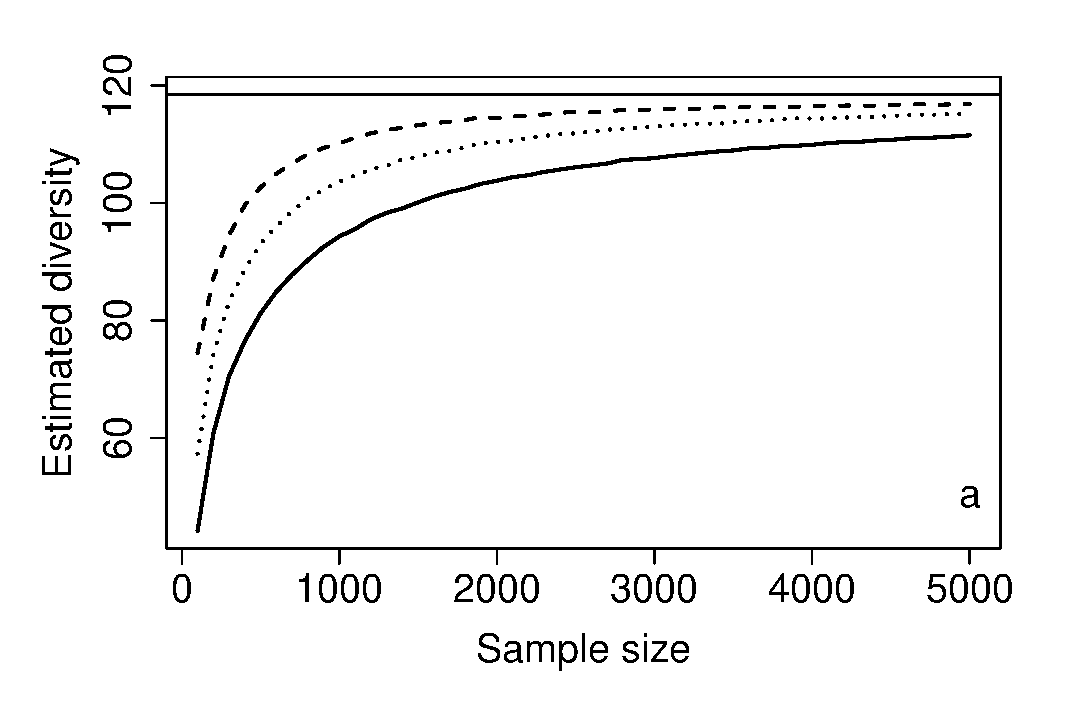
\includegraphics[width=.8\textwidth]{Fig1}}

Les tableaux et figures sont appelés par les commandes du type \code{\textbackslash tableSC}. Le préfixe est \code{table} ou \code{figure}, le suffixe:
\begin{itemize}
  \item \code{SC} (figure~\ref{fig:sc}) pour \foreignlanguage{english}{Side Caption}: l'objet est placé dans le texte (sa largeur par défaut est 80\% de la largeur de la colonne), la légende est dans la marge. Le placement par défaut est \code{[htbp]}.

\tableFW{tab:FW}
{Notations des effectifs, tableau espèces-communautés.}
{
\begin{tabularx}{\textwidth}{p{2cm} p{7cm} p{1cm} X}
\toprule
 & Communauté $i$ & $\dots$ & Total: méta-communauté \\

\midrule
Espèce $s$ 
   & $n_{si}$: nombre d'individus de l'espèce $s$ dans la communauté $i$. \newline
  $\hat{p}_{si}=n_{si}/n_{+i}$ est l'estimateur de la probabilité $p_{si}$ qu'un individu de la communauté $i$ soit de l'espèce $s$.
  &
  & $n_{s+}=\sum_i{n_{si}}$ \newline
    $p_s=\sum_i{w_{i}p_{si}}$ \\

$\dots$
  &
  &
  & \\

Total
  & $n_{+i}$: nombre d'individus de la communauté.\newline 
    $w_i$: poids de la communauté
  &
  & $n$: nombre total d'individus échantillonnés \\

\bottomrule
\end{tabularx}
}

  \item \code{FW} (tableau~\ref{tab:FW}) pour \foreignlanguage{english}{Full Width}: l'objet occupe toute la largeur de la page (hors marges d'impression), la légende est dans le texte, au dessus pour les tableaux, au-dessous pour les figures. Le placement par défaut est \code{[tbp]}.

\figureMargin{fig:Margin}
  {Figure dans la marge (\code{\textbackslash figureMargin})}
  {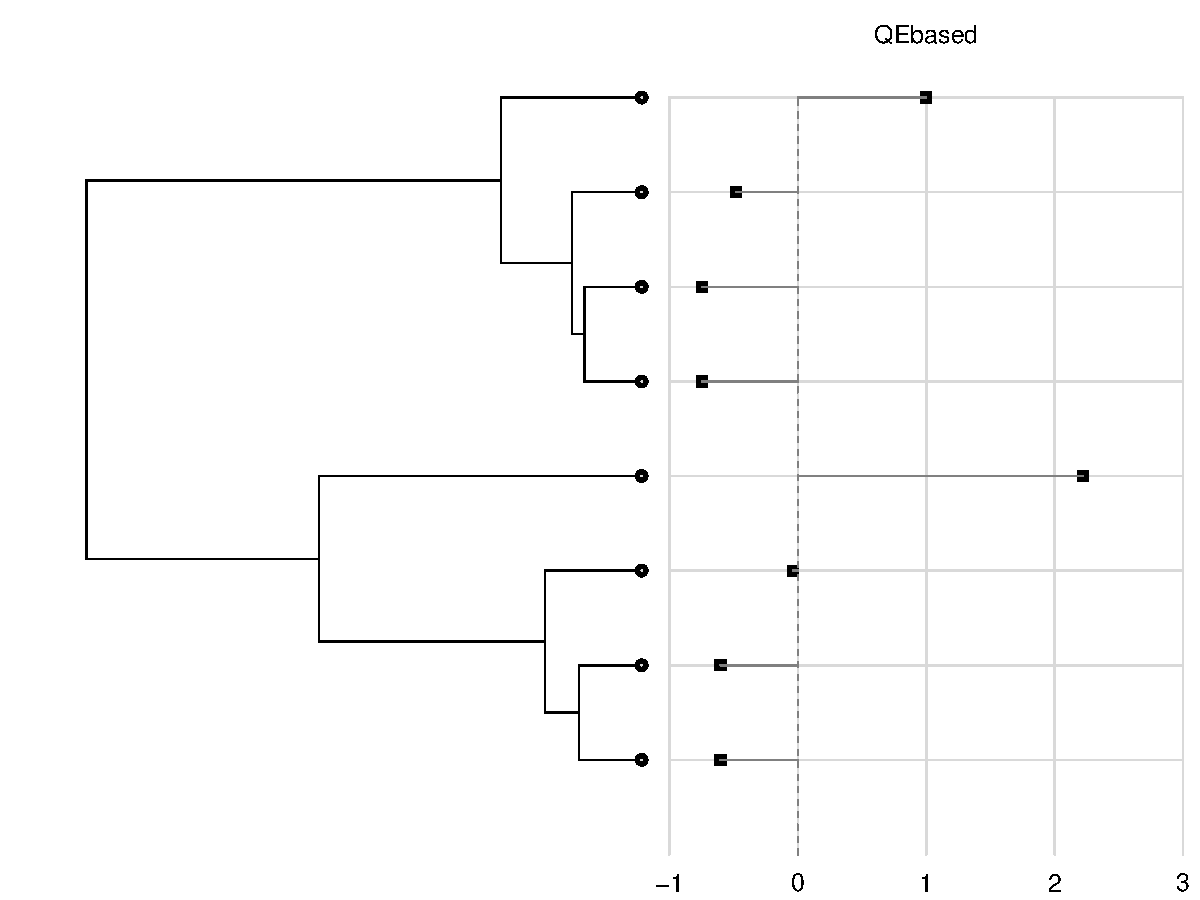
\includegraphics[width=\textwidth]{Fig2}}

  \item  \code{Margin} (figure~\ref{fig:Margin}) pour placer l'objet et sa légende dans la marge.
\end{itemize}

\figureFW{fig:subfig}
{Figure multiple. La commande \code{\textbackslash includegraphics} est simplement remplacée par les commandes \code{\textbackslash subfloat}}
{
  \subfloat[Première sous figure. \label{fig:subfiga}]
    {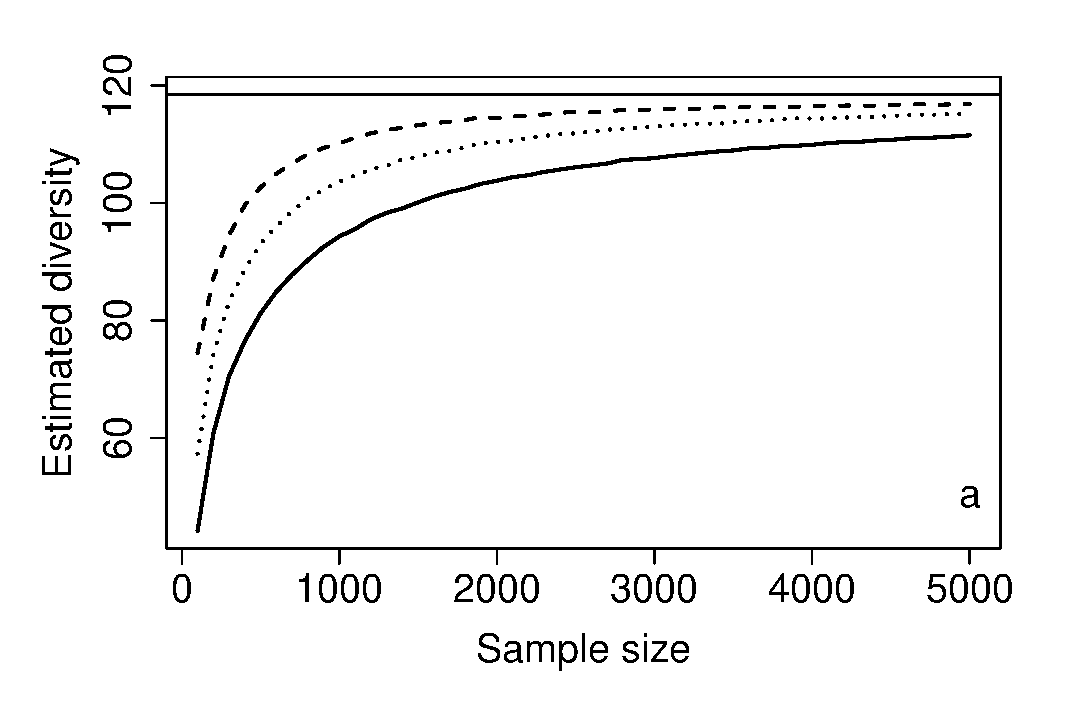
\includegraphics[width=.45\textwidth]{Fig1}}
	\hfill
  \subfloat[Deuxième sous figure. \label{fig:subfigb}]
    {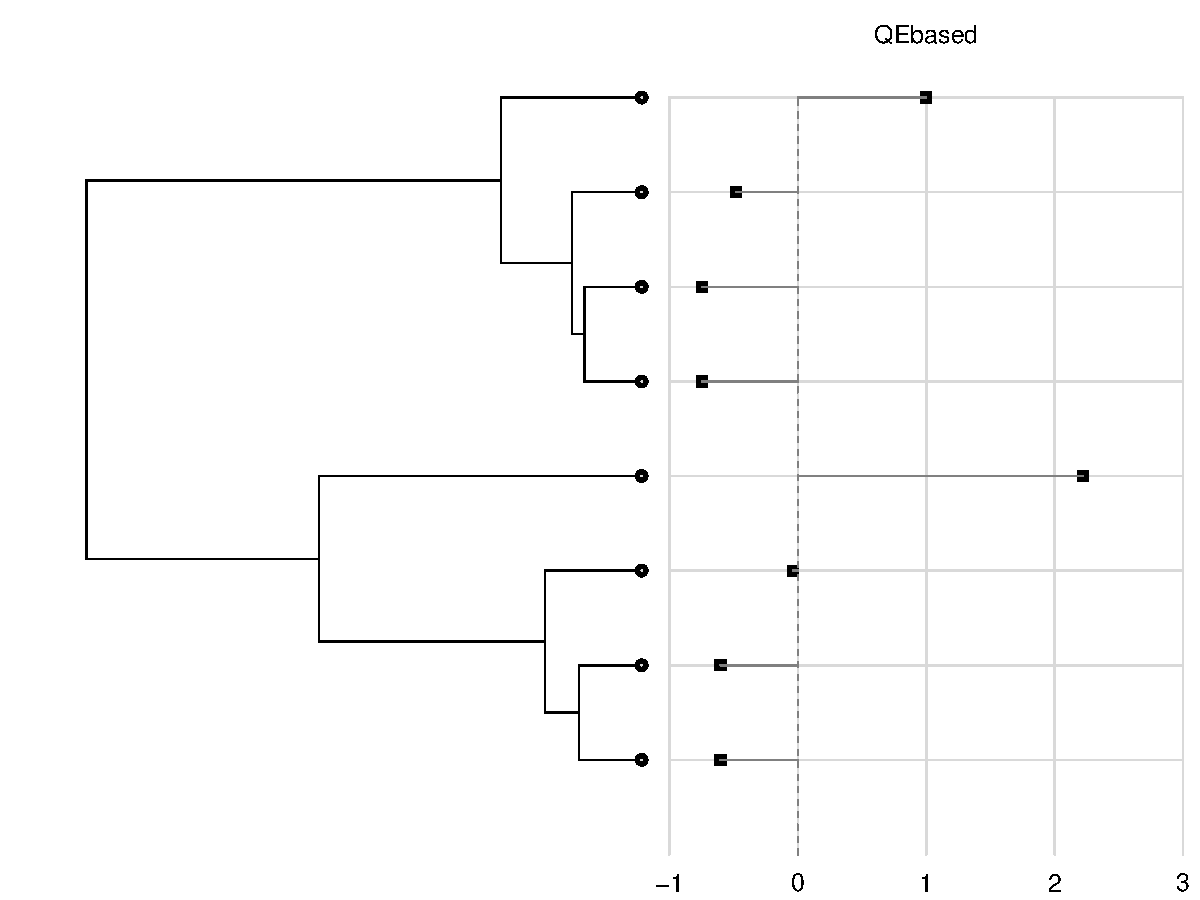
\includegraphics[width=.45\textwidth]{Fig2}}
}

La syntaxe des six commandes est identique, avec 4 paramètres dont trois obligatoires:
\begin{itemize}
  \item paramètre optionnel (ignoré pour les objets dans la marge): placement, par défaut \code{[htbp]} ou \code{[tbp]}.
  \item étiquette de l'objet.
  \item légende
  \item contenu de l'objet, en général un tableau, \code{\textbackslash includegraphics} ou un bout de code R si knitr est utilisé. Le package \code{subfig} permet des figures multiples (figure~\ref{fig:subfig}), de préférence en pleine largeur.
\end{itemize}


\subsubsection{Encadrés}

Les encadrés sont créés par le package \code{bclogo}: voir sa documentation pour plus de détail.

\begin{bclogo}[logo=\bctrombone, noborder=true, couleur=lightgray!50]{Encadré}
  \lipsum[2]
\end{bclogo}


\subsection{Notes}

Les notes sont appelées par \code{\textbackslash footnote} mais sont affichées en marge\footnote{Exemple de note de \og bas de page\fg{}}.

Le code informatique utilisé dans des bouts de code R (\foreignlanguage{english}{\emph{chunks}}) peut être placé en bas de page en utilisant \code{\textbackslash verbfootnote} \verbfootnote{
\scriptsize
Code R:

> 2+2

[1] 4
}
.


\section{Commandes}

\subsection{Nouvelles commandes}

Les nouvelles commandes suivantes sont incluses dans le modèle:
\begin{itemize}
  \item \code{\textbackslash Var} pour la variance, en mode mathématique: $\Var(X)=\nicefrac{\sum_i(x_i-\bar{x})^2}{(n-1)}$,
  \item \code{\textbackslash code\{\}} pour afficher du code dans le texte. Attention, le code est insécable et peut provoquer des dépassements de largeur de ligne (\foreignlanguage{english}{``Overfull hbox''}) si leur retour à la ligne cause un espacement trop important entre les mots. Forcer le retour à la ligne en insérant \code{\textbackslash break} avant le code.
\end{itemize}

\subsection{Equations}

Utiliser les environnements \code{\textbackslash equation} ou \code{\textbackslash multline}:

\begin{multline}
  \tilde{H}
  = -\sum_{s=1}^{s^{n}_{\ne 0}}
    {\frac{n_s}{n}\left(\mathrm{\Psi}\left(n\right) - \mathrm{\Psi}\left(n_s\right)\right)} \\
    -\frac{s_{1}}{n} {\left(1-A\right)}^{1-n} \left(-{\ln\left(A\right)}-\sum^{n-1}_{r=1}{\frac{1}{r}{\left(1-A\right)}^r}\right)
\label{eq:Chao2013}
\end{multline}

 \code{\textbackslash align} permet de présenter les calculs en plusieurs lignes:

\begin{align}
  ^{q}\bar{H}_{\beta}\left(T\right)
    &= \sum_i{w_i}\sum_k{\frac{T_k}{T}{^{q}_{ik}H}}\\
    &= \sum_i{w_i}\sum_k{\frac{T_k}{T}\sum_u{p^{q}_{kui}\ln_q\frac{p_{kui}}{p_{ku}}}}
\end{align}



\section{Bibliographie}

Les références bibliographiques doivent être appelées par la commande \code{\textbackslash autocite}. 
Elles sont affichées en marge \autocite{Rao1985} et dans le récapitulatif en fin de document.
La commande \code{\textbackslash textcite} permet d'intégrer le nom des auteurs dans le texte, par exemple \textcite{Rao1985}.

\newpage 
\textit{Page vide pour la démonstration des références bibliographiques.}
\newpage 
Les références répétées \autocite{Pelissier2001} sont traitées.
Une répétition immédiate est remplacée par \textit{Ibid.} \autocite{Pelissier2001}
Une répétition sur la même (double) page séparée par une autre citation \autocite{Rao1985} est réduite au nom de l'auteur et à l'année \autocite{Pelissier2001}.
Une répétition au delà de la double page affiche en plus le titre et un renvoi vers la page de la première citation \autocite{Rao1985}.


\section{Historique}

\paragraph{Version 1.14}
Logo EcoFoG version 2021.

\paragraph{Version 1.13}
Logo EcoFoG version 2020.

\paragraph{Version 1.11}
Suppression des couvertures de thèse et HDR (utiliser le modèle TheseHdrUG).
Ajout d'une couverture PDF.
Retour à bibtex: plus rapide, plus pratique avec TeXstudio.

\paragraph{Version 1.10}
Logo EcoFoG version 2017.

\paragraph{Version 1.9}
Gestion des DOI.

\paragraph{Version 1.8}
Le moteur de bibliographie est maintenant Biber au lieu de Bibtex.

\paragraph{Version 1.7}
Support de \code{\textbackslash textcite} et améliorations internes.

\paragraph{Version 1.6}
Deux pages de garde possibles: rapport ou thèse/HDR.

\paragraph{Version 1.4}
Logo EcoFoG version 2015.

\paragraph{Version 1.3}
Support des sous-figures et meilleure gestion des références bibliographiques répétées.

\paragraph{Version 1.2}
Première version diffusée.

%%%------------------------------------------------------------------------------
\backmatter
\clearpage

%%% BIBLIOGRAPHY
%%% -------------------------------------------------------------

% Marges étroites
\SmallMargins

% Si la bilbiographie est longue, police plus petite et deux colonnes
%\twocolumn
%\renewcommand*{\bibfont}{\scriptsize}

\printbibliography

% Pour intégrer la quatrième de couverture du domument Couverture.pdf (commenter les deux lignes sinon):
\evenpage

\includepdf[pages={4}]{Couverture.pdf} 


\end{document}
